\documentclass{article}
\usepackage[utf8]{inputenc}
\usepackage{amsmath}
\usepackage{tikz}
\usetikzlibrary{trees}
\usepackage{qtree}
\usepackage{comment}
\usepackage[dvipsnames]{xcolor} % Colors

\begin{document}

\section*{\small 3.2 Justifica l’ambigüitat o no ambigüitat de les següents $CFG$’s:}

\textbf{e)}

\begin{tabular}{rcl}
$S$ & $\rightarrow$ & AaBA $\mid$ ABaA $\mid$ ACA $\mid$ AbabA \\
$B$ & $\rightarrow$ & bb \\
$C$ & $\rightarrow$ & Bb \\
$A$ & $\rightarrow$ & aA $\mid$ bA $\mid$ $\lambda$ \\
\end{tabular}

\vspace{1em}

\noindent El mot \(abba\) es pot generar amb dos arbres de derivació diferents:

\vspace{1em}

\noindent
\begin{minipage}{0.48\textwidth}
\centering

%\textbf{Arbre 1 ($abba$):}
\[
\begin{tikzpicture}
  \Tree
  [.$S$
    [.$A$
      [.$\lambda$ ]
    ]
    [.$a$ ]
    [.$B$
      [.$bb$ ]
    ]
    [.$A$
      [.$aA$
        [.$\lambda$ ]
      ]
    ]
  ]
\end{tikzpicture}
\]
\end{minipage}
\hfill
\begin{minipage}{0.48\textwidth}
\centering

%\textbf{Arbre 2 ($abba$):}
\[
\begin{tikzpicture}
  \Tree
  [.$S$
    [.$A$
      [.$aA$
        [.$\lambda$ ]]]
    [.$B$
      [.$bb$ ]
    ]
    [.$a$ ]
    [.$A$
      [.$\lambda$ ]
    ]
  ]
\end{tikzpicture}
\]
\end{minipage}

\vspace{1em}
\vspace{1em}
\vspace{1em}
\vspace{1em}
\vspace{1em}
\vspace{1em}
\vspace{1em}
\vspace{1em}

\noindent Com que hi ha dos arbres de derivació diferents per a la mateixa paraula $abba$, la gramàtica és \textbf{ambigua}.

\vspace{1em}

\noindent \textcolor{OliveGreen}{\textbf Cal recordar que els camins de derivació de cada descomposició \textbf{no demostren l'ambigüitat}, però són útils per aclarir el procés de derivació d'un mot.}

\begin{comment}    

\noindent Els camins de derivació de cada descomposició són els següents \textbf{No demostren l'ambigüitat}, però són útils per aclarir el procés de derivació d'un mot:

\begin{align*}
S &\xRightarrow[S \to AaBA]{} AaBA \\
   &\xRightarrow[A \to aA]{} aBA \\
   &\xRightarrow[B \to bb]{} abbA \\
   &\xRightarrow[A \to \lambda]{} abba
\end{align*}

\begin{align*}
S &\xRightarrow[S \to ABaA]{} ABaA \\
   &\xRightarrow[A \to aA]{} aBaA \\
   &\xRightarrow[B \to bb]{} abbaA \\
   &\xRightarrow[A \to \lambda]{} abba
\end{align*}
\vspace{1em}
\end{comment}

\end{document}
